%!TEX root = problems.tex

\printanswers

\begin{questions}

\question
Create three nodes in Cypher to represent three friends -- Jack, Jerry and John.
\begin{solution}
  \begin{minted}{cypher}
CREATE
  (jack:User:Male {Name: "Jack"}), 
  (jerry:User:Male {Name: "Jerry"}),
  (john:User:Male {Name: "John"})

RETURN
  jack, jerry, john;
  \end{minted}
\end{solution}
  
\question
Create relationships showing that:

\begin{itemize}
  \item Jack follows Jerry on Twitter.
  \item Jack follows John on Twitter.
  \item John follows Jerry on Twitter.
\end{itemize}

\begin{solution}
  \begin{minted}{cypher}
MATCH
  (n:User {Name: "Jack"}), (m:User {Name: "Jerry"})
CREATE
  (n)-[r:FOLLOWS_TWITTER]->(m)
RETURN r;
// OR create two/three at a time:
MATCH 
  (n:User {Name: "Jack"}),
  (m:User {Name: "Jerry"}),
  (p:User {Name: "John"})
CREATE
  (n)-[r:FOLLOWS_TWITTER]->(p),
  (p)-[s:FOLLOWS_TWITTER]->(m)
RETURN
  r, s;
  \end{minted}
\end{solution}

\question
Add some information about Jack, Jerry and John:
\begin{itemize}
  \item Jack joined Twitter in May 2010.
  \item Jerry joined Twitter in June 2012.
  \item John joined Twitter in January 2016.
\end{itemize}

\begin{solution}
\begin{minted}{cypher}
MATCH (a:User {Name: "Jack"})
SET a.joinTwitter = "May 2010"
RETURN a;

MATCH
  (a:User {Name: "Jerry"})
  , (b:User {Name: "John"})
SET
  a.joinTwitter = "June 2012"
  , b.joinTwitter = "January 2016"
RETURN
  a, b;
  \end{minted}
\end{solution}

\question
Add some information about the following relationships:
\begin{itemize}
  \item Jack started following Jerry in July 2012.
  \item Jack started following John in February 2016.
  \item John started following Jerry on January 2016.
\end{itemize}

\begin{solution}
  \begin{minted}{cypher}
MATCH
  (a:User {Name: "Jack"})-[r:FOLLOWS_TWITTER]->(b:User {Name: "Jerry"})
SET
  r.started = "June 2012";
	
MATCH
  (a:User {Name: "Jack"})-[r:FOLLOWS_TWITTER]->(b:User {Name: "John"})
SET
  r.started = "February 2016";
	
MATCH
  (a:User {Name: "John"})-[r:FOLLOWS_TWITTER]->(b:User {Name: "Jerry"})
SET
  r.started = "January 2016";
  \end{minted}
\end{solution}

\question
  Create the following graph in Cypher:
  \begin{center}
  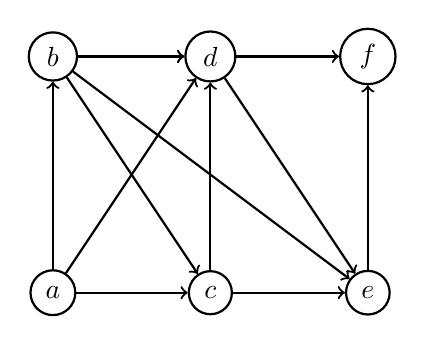
\begin{tikzpicture}
    \begin{scope}[every node/.style={circle,thick,draw}]
      \node (a) at (0,0) {$a$};
      \node (b) at (0,3) {$b$};
      \node (c) at (2,0) {$c$};
      \node (d) at (2,3) {$d$};
      \node (e) at (4,0) {$e$};
      \node (f) at (4,3) {$f$};
    \end{scope}
    \begin{scope}[every edge/.style={draw=black,thick}]
      \path (a) edge[->] (b);
      \path (a) edge[->] (c);
      \path (a) edge[->] (d);
      \path (b) edge[->] (c);
      \path (b) edge[->] (d);
      \path (b) edge[->] (e);
      \path (b) edge[->] (d);
      \path (c) edge[->] (d);
      \path (c) edge[->] (e);
      \path (d) edge[->] (e);         
      \path (e) edge[->] (f);
      \path (d) edge[->] (f);
    \end{scope}
  \end{tikzpicture}
  \end{center}
\begin{solution}
Left for the student.
\end{solution}




\end{questions}

%\begin{thebibliography}{9}
%
%\bibitem{biggs02}
%  Norman Biggs,
%  \emph{Discrete Mathematics},
%  Oxford University Press,
%  2nd edition,
%  2002.
%\end{thebibliography}
